\chapter[Implementering af hardware]{Hardware}
\mnote{Nick Østergaard}

% Vi skriver her om hvordan vi faktisk realiserer det vi har sankket
% om i Hardwaredesignet

\section{Mikroprocessor}
\label{sc:i-mcu}
Vi har som beskrevet i afsnit~\vref{sc:d-mikroprocessor}, at vi
anvender en \texttt{atmega128} som hjernen i maskinen. Det kræver, at
der laves et print, hvor vi kan tilslutte alle maskinens enheder. I
stedet for at lave vores eget har vi brugt~\cite{fronter:atmega128}.

Der er ved brug af dette MCU print én ting, som man skal være
opmærksom på. De er ikke nogen strømforsyning i printet, hvlket vil
sige, at den skal have en 5V forsyning fra en af de periferi endheder
den tilsluttets. Dette løser vi med vores stepmotor dirver print.

\section{Stepmotor driver}
\label{sc:stepmotor-driver}

\mnote{
  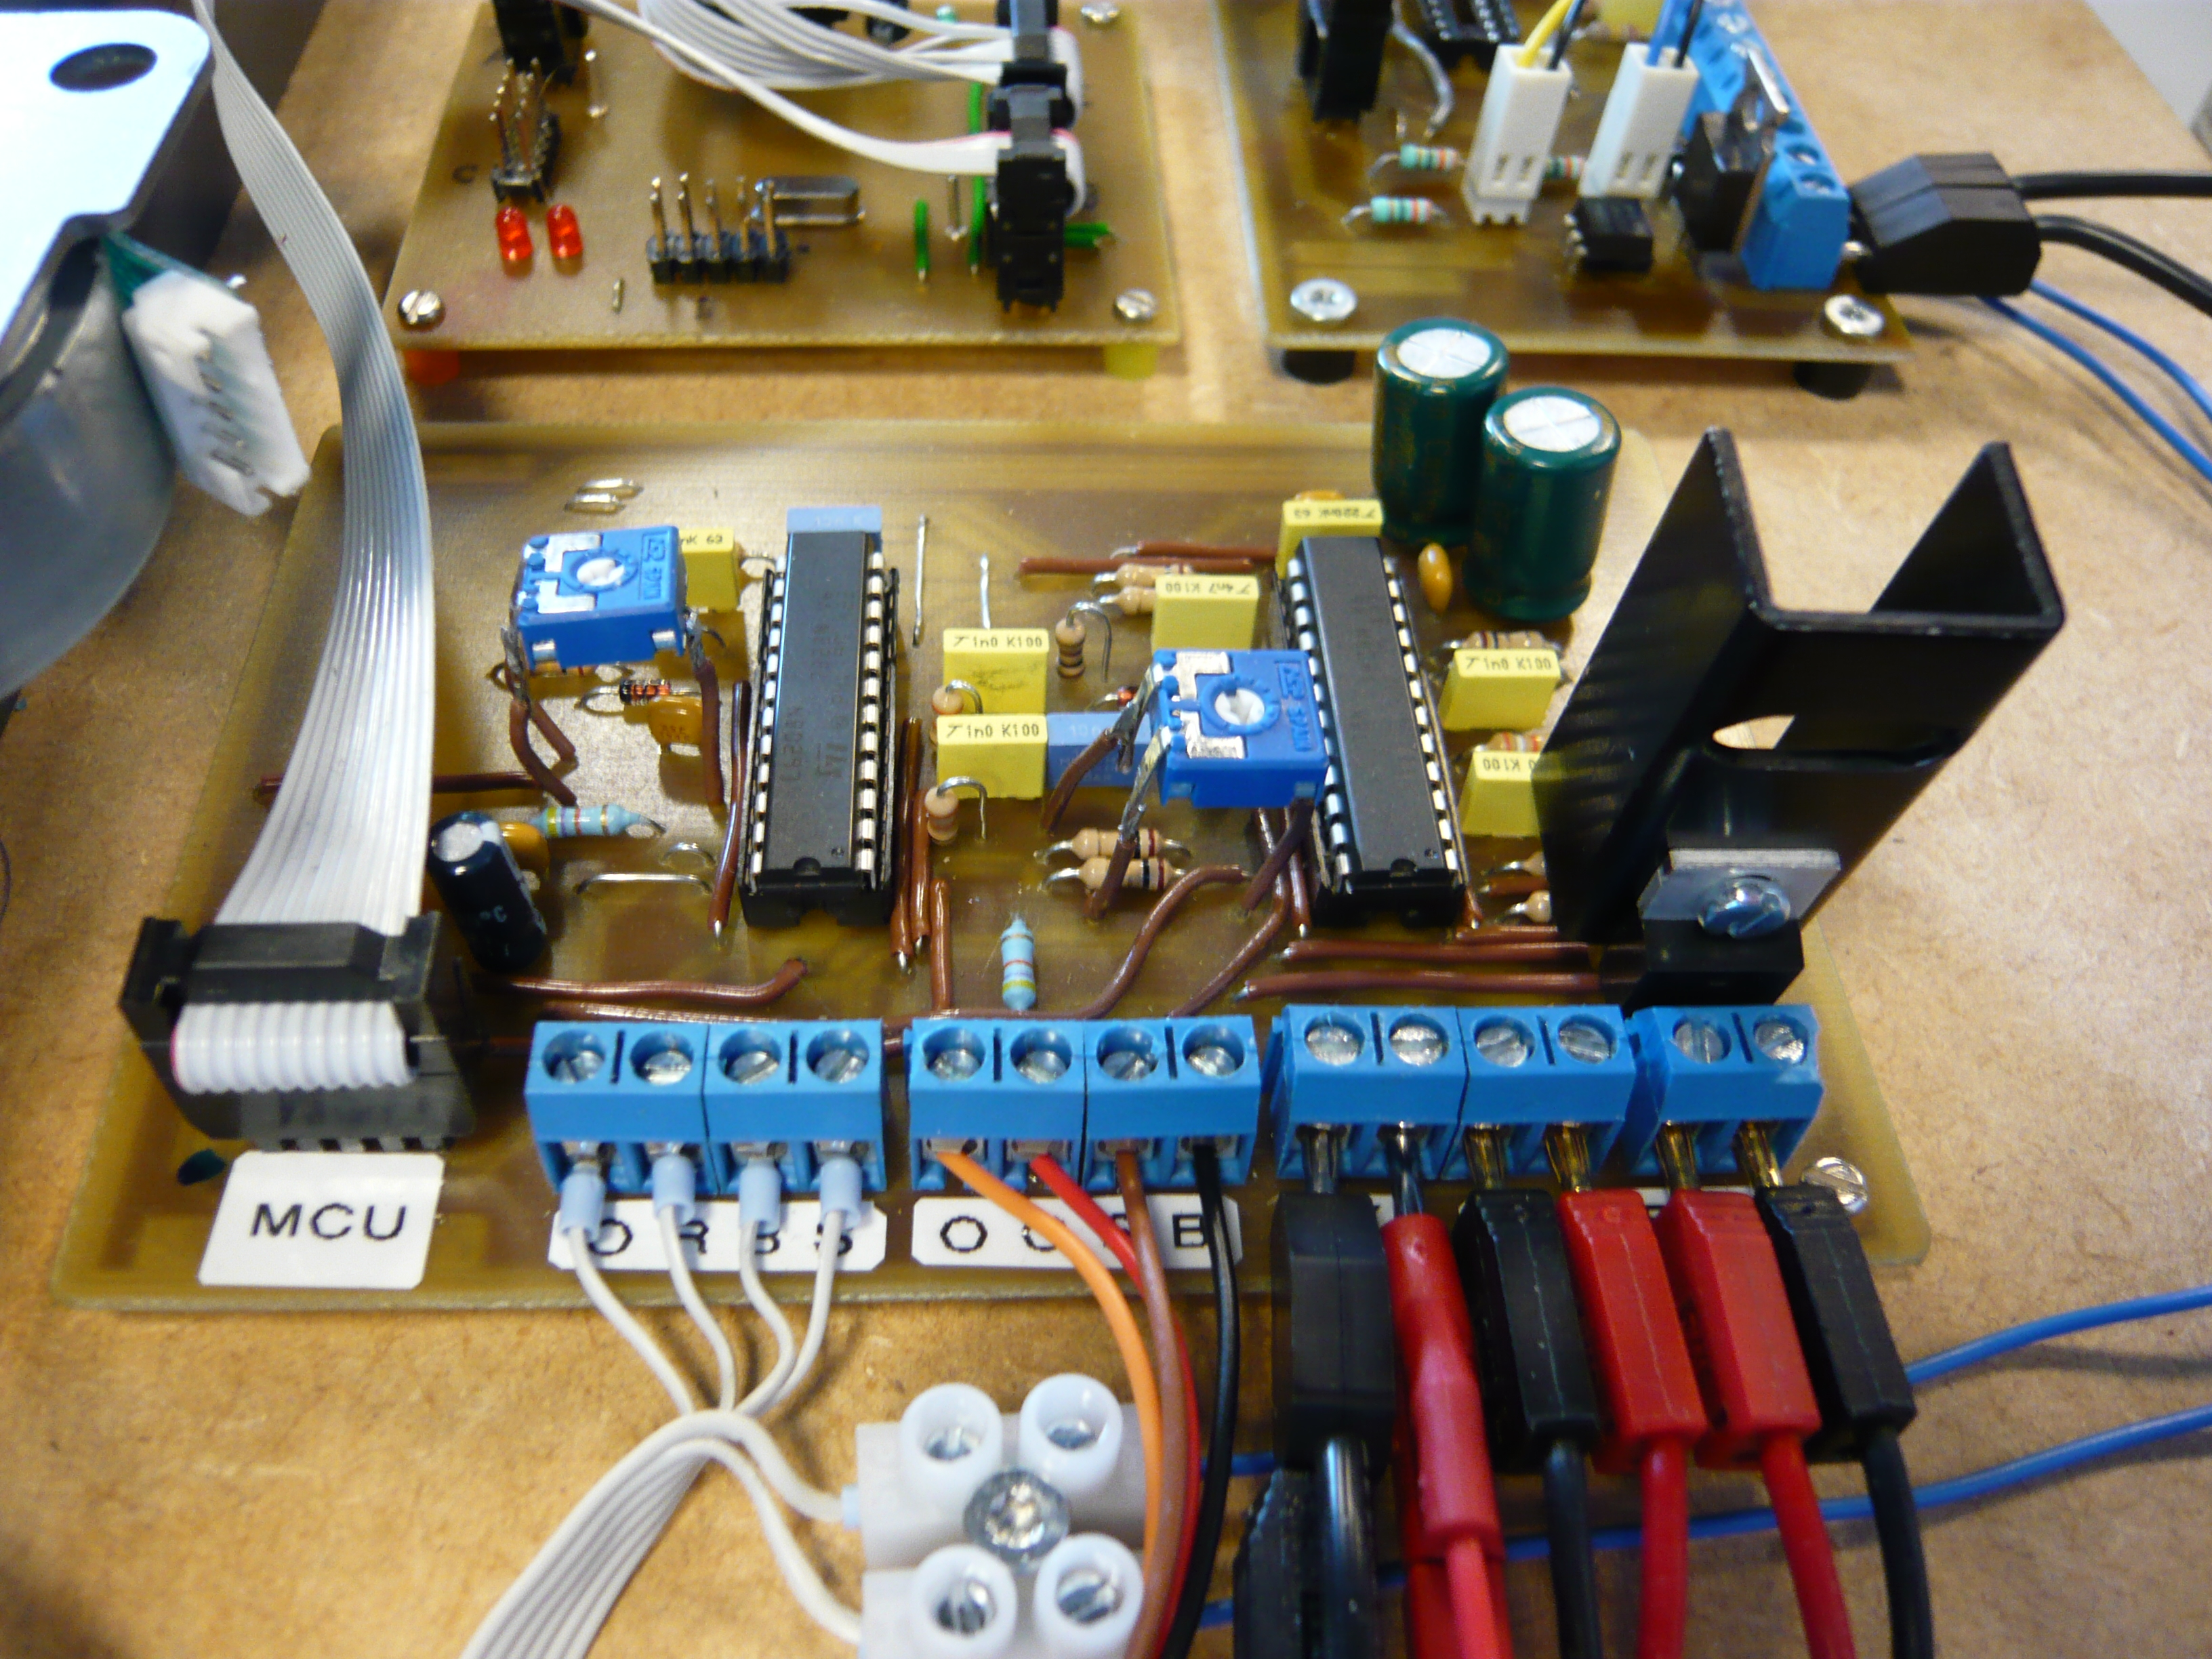
\includegraphics[width=\marginparwidth]{./img/stepmotordriver}
  \captionof{figure}{Stepmotor driver}
  \label{fig:stepdriver}
}

Vi konstruerer en stepmotor driver med et par integrerede stepmotor
drivere. Mere specefikt anvender vi en L6208N, som kan styre en
bipolar stepmotor. Vi bruger denne driver kreds, da den er simpel at
styre, samt der er mulighed for at lave strømbegrænsning. Hvilket vil
gøre, at vi kan skrue forsyningsspændingen til motorerne op og
begrænse strømmen, således motorerne er mere kvik, hvilket betyder at
vi kan køre hurtigere. Hvilket igen vil være en fordel, da motorene er
gearet ned.

\mnote{
  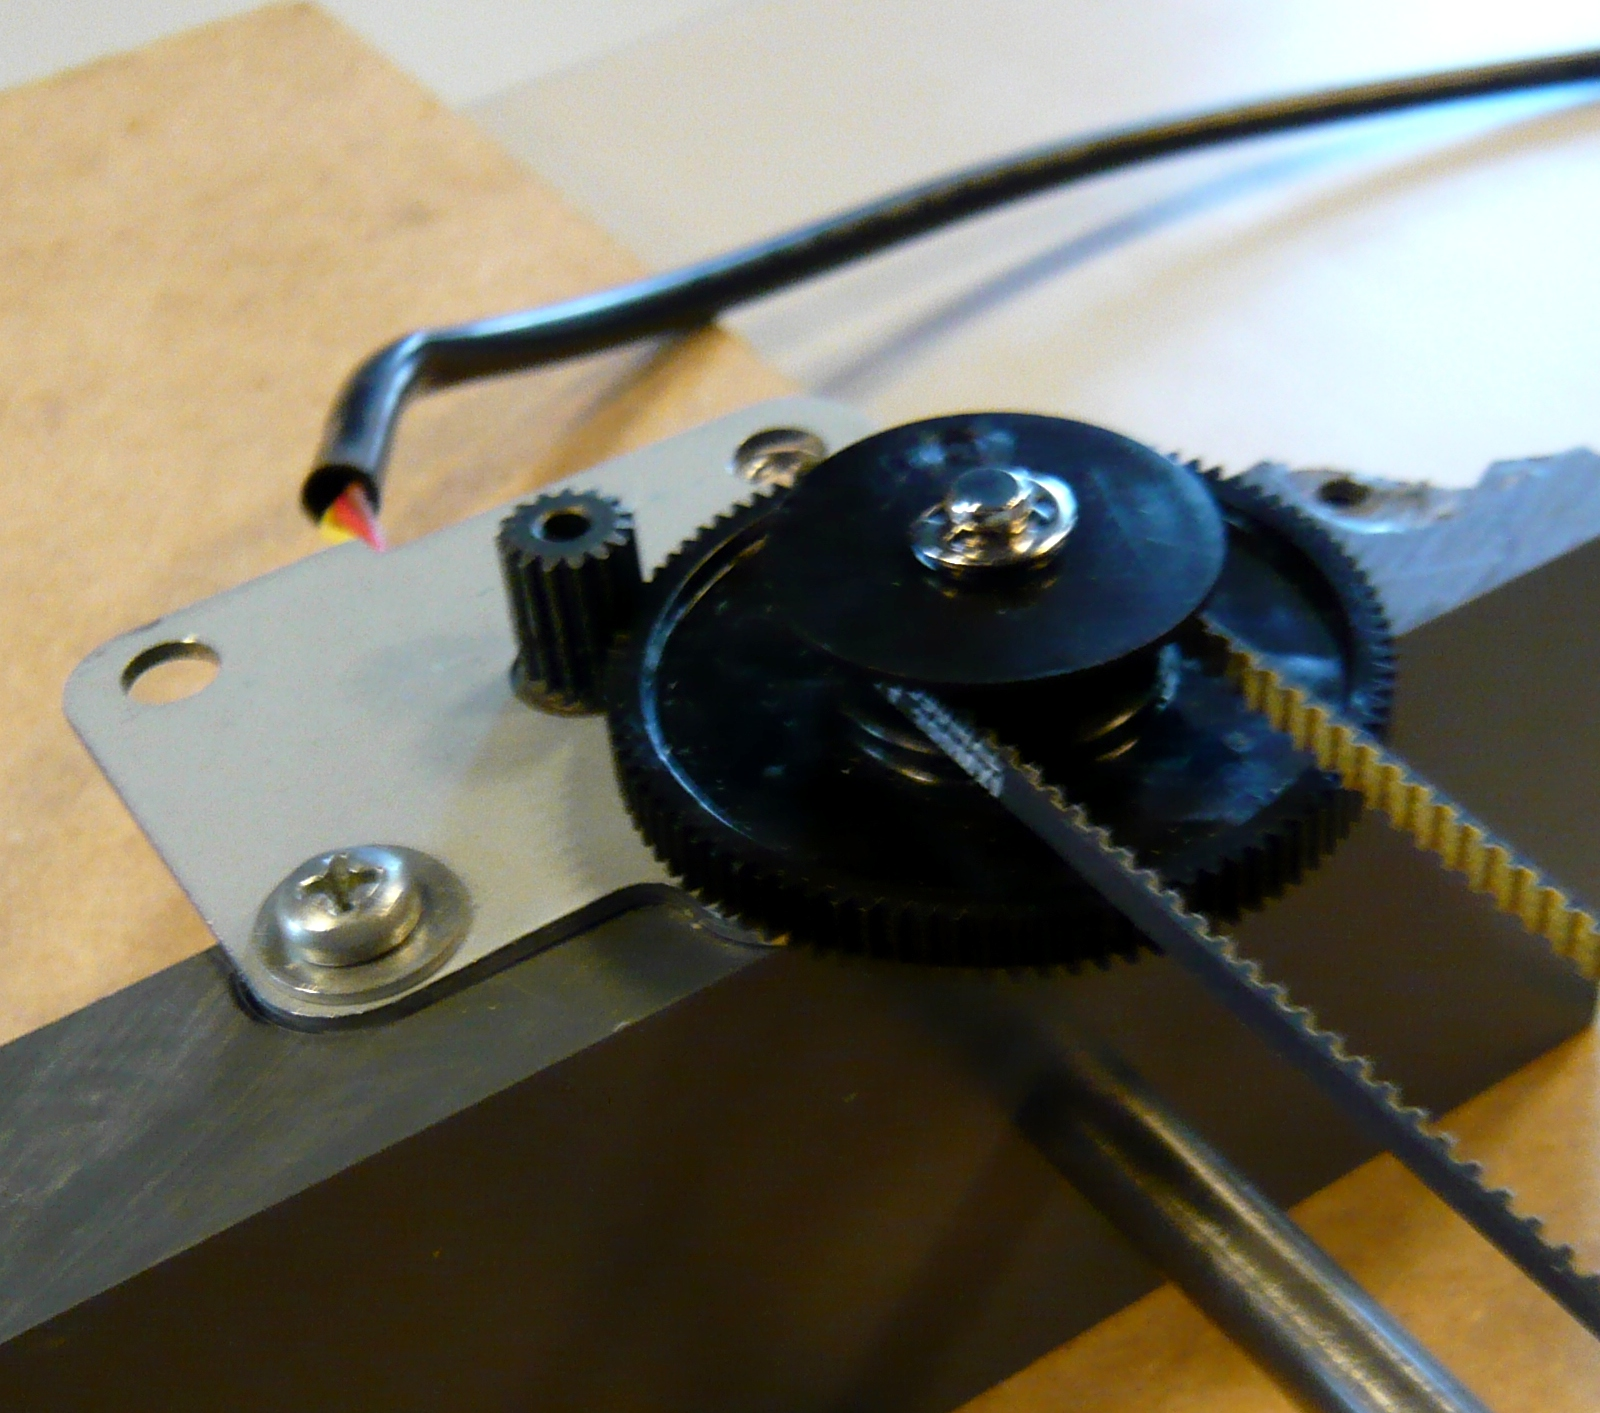
\includegraphics[width=\marginparwidth]{./img/x-motor}
  \captionof{figure}{X-aksens motor monteret}
  \label{fig:x-motorimg}
}

\mnote{
  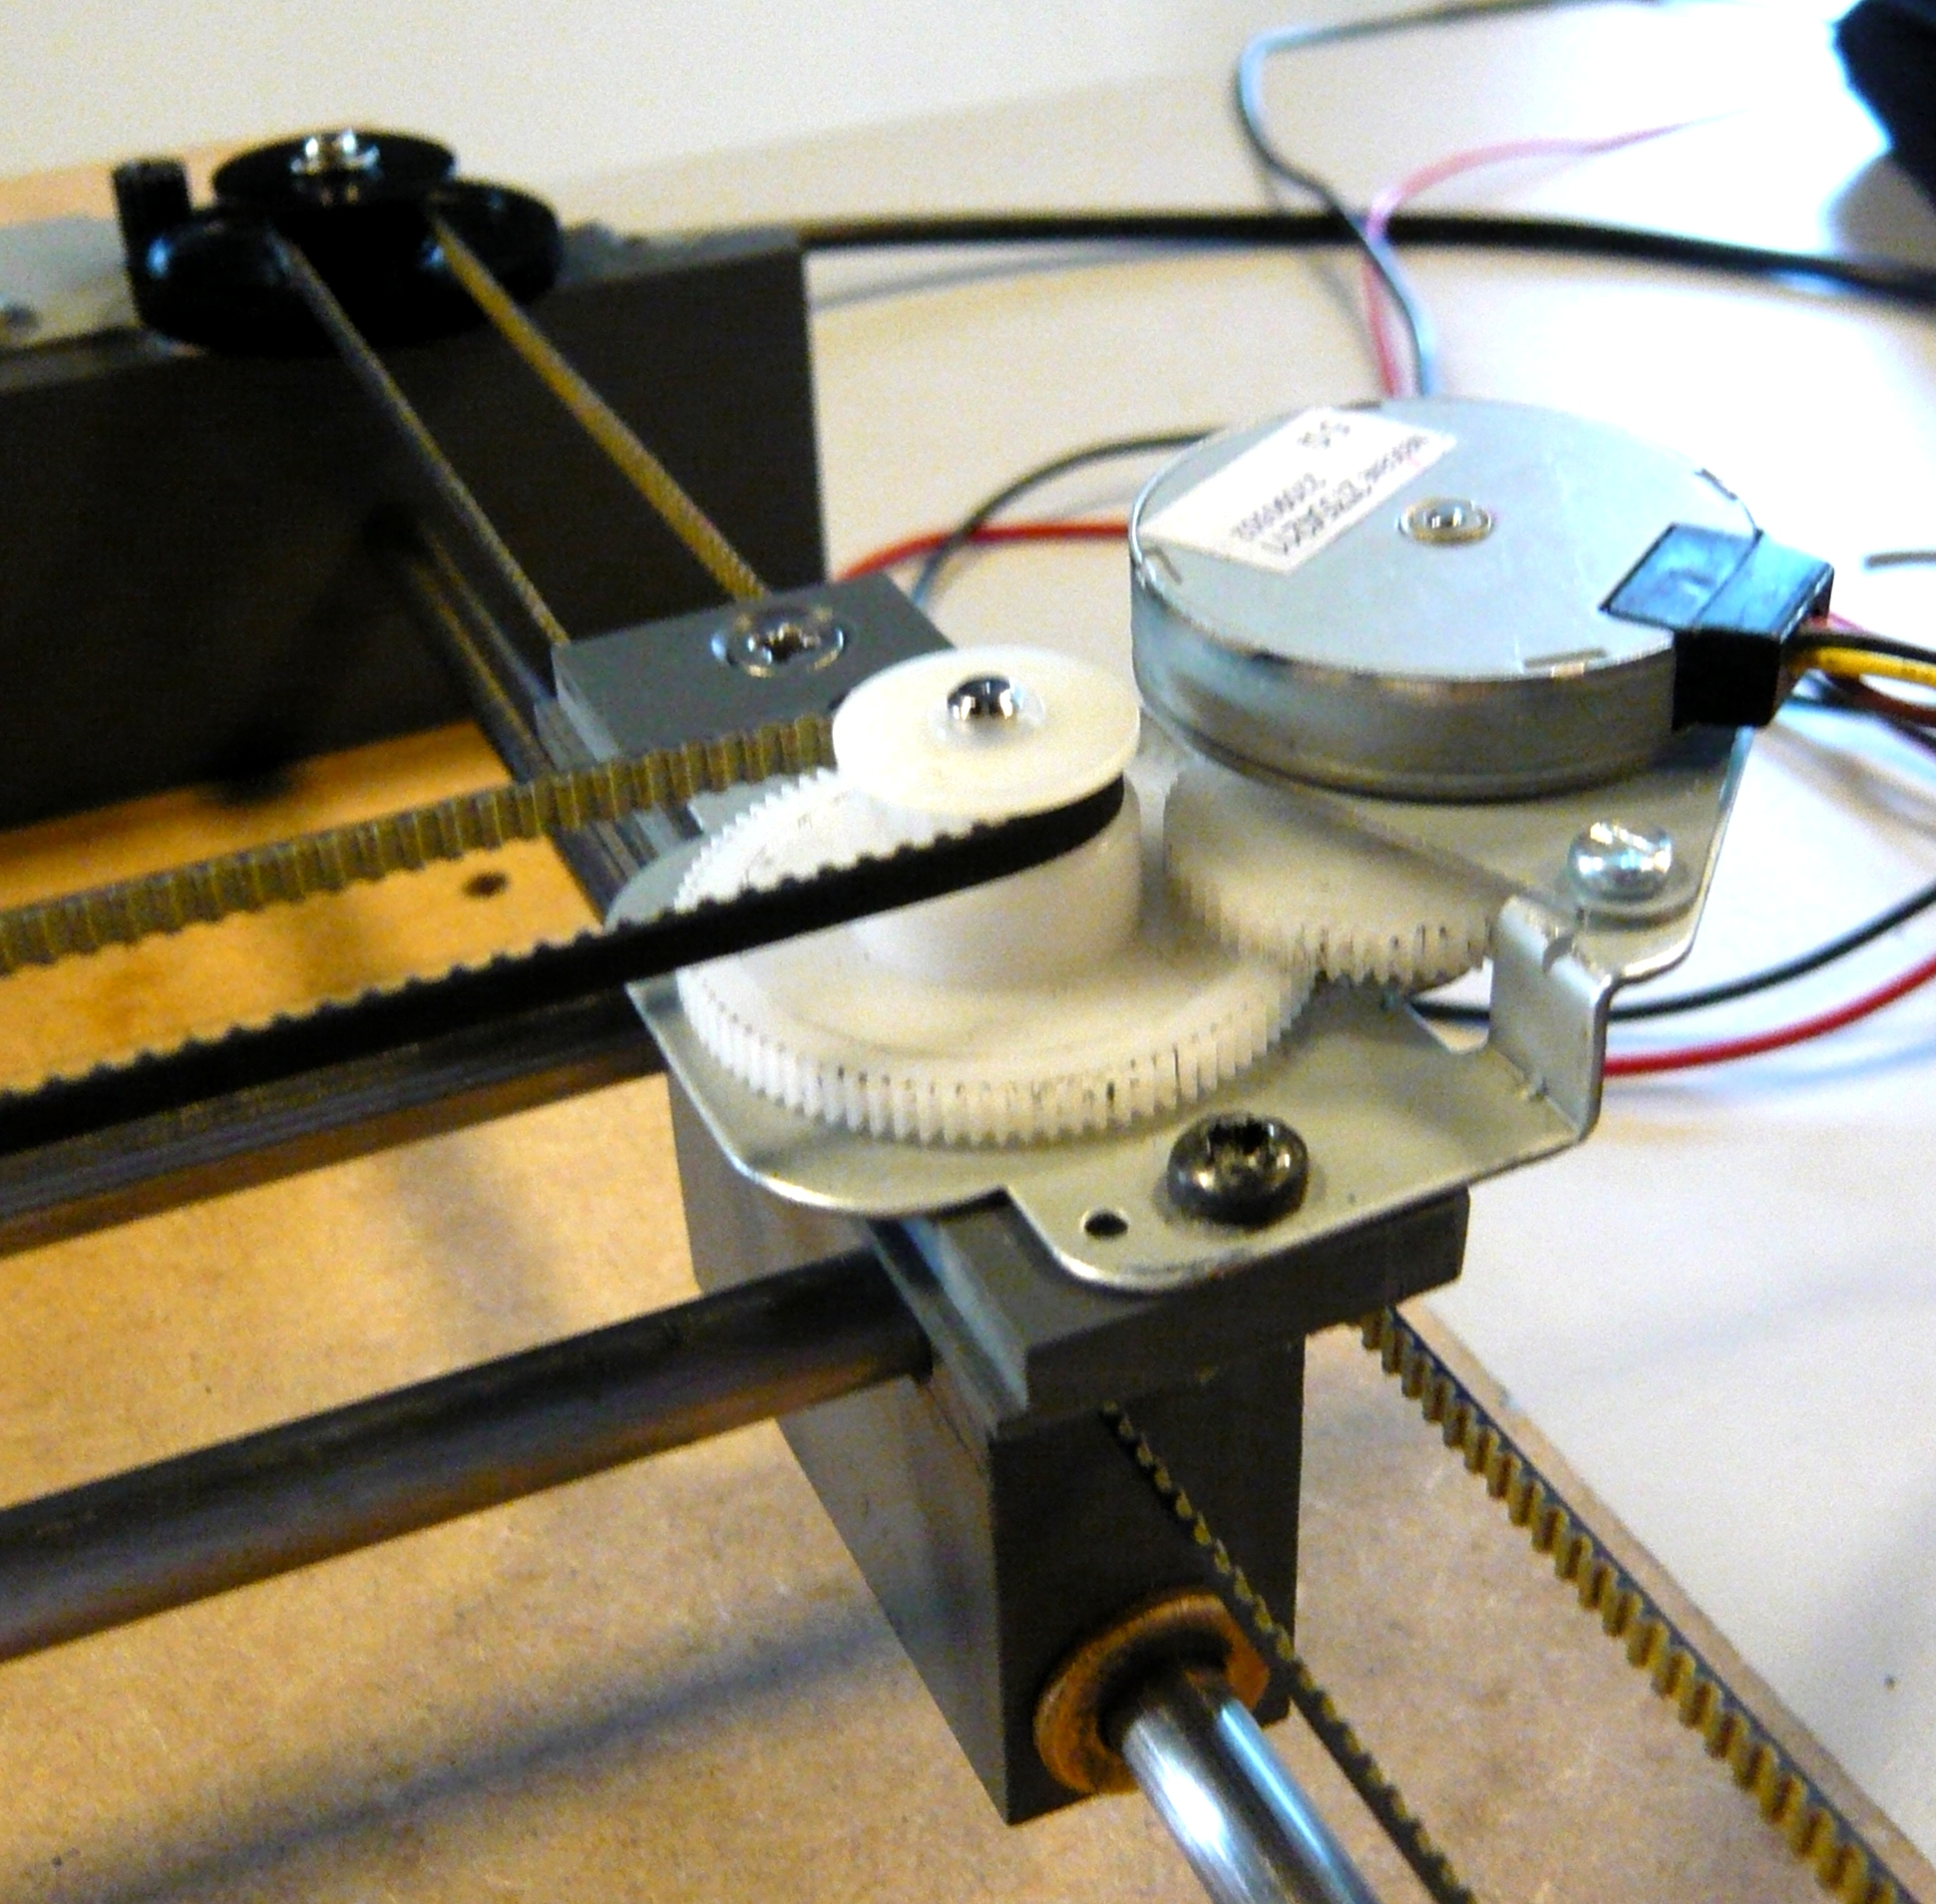
\includegraphics[width=\marginparwidth]{./img/y-motor}
  \captionof{figure}{Y-aksens motor monteret}
  \label{fig:y-motorimg}
}

For at styre driveren, skal vi blot styre den ved at sætte nogle input
høje eller lave. Man kan bestemme om den skal køre half step eller
full step ved at sætte et signal høj eller lav. Man sætter et signal
højt, for at tage ét skridt. Ligeledes kan man også styre hvilken
retning motoren skal dreje, afhængig af om inputtet til driveren er
høj eller lav. Det fulde diagram kan ses i bilag~\vref{b-l6208n}.

De relevante inputs til driver kredssen er skal anvende på følgende måde:

\begin{itemize} \firmlist
\item \texttt{HALF/FULL} Logisk høj for at køre half step
  og lav for full step
\item \texttt{CW/CWW} Logisk høj sætter den til at køre med uret mens
  logisk lav sætter den til at dreje mod uret
\item \texttt{CLOCK} Logisk høj i minimum $1\mu s$ for at tage ét skridt
\item \texttt{RESET} Skal sættes logisk høj under kørsel af motor, da
  logisk lav vil resette fase stillingen
\item \texttt{ENABLE} Skal sættes logisk høj for at åbne for strømmen
  gennem den indbyggende H-bro, og lav for at afbryde for strømme
\end{itemize}

Det skal noteres, at der er på det fulde hardware diagram i
bilag~\vref{b-l6208n} er en \texttt{DECAY} forbindelse, som ikke er
nødvendig at tage stilling til. Den kontrollerer blot hvilen vej
tilbageslagsstrømmen kan løbe, når motoren skifter skridt.

De to potentiometre \texttt{RV1} og \texttt{RV2} danner en
spændingsdeler med hver sin seriemodstand, som bruges til den interne
strømbegrænser. Her bruger vi en 5V sændingsregulator til at få en
stabil spænding til denne spændingsreference. Og som nævnt i
afsnit~\vref{sc:i-mcu} har vi brug for en ekstern spændingsforsyning
gennem en IO port. Det er her vi har forsyningsspændingen til vores
MCU og andre perifære enheder.

\section{Sensorer}
Som beskrevet i afsnit~\vref{sc:sensorer} vil vi anvende et par
fotogafler, til at detektere aksernes nulstillings position.

\mnote{
  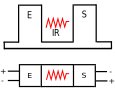
\includegraphics[width=\marginparwidth]{./img/fotogaffel}
  \captionof{figure}{Skitse af fotogaffel}
  \label{fig:fotogaffel}
}

En fotogaffel virker som en elektrisk kontakt. Den er opbygget af en
lysdiode, typisk en infrarød lysdiode, og en transistor. Lyser man på
en åben transistor, vil den lede strøm gennem collector og
emitter. Slukker man lyset vil den ikke lede. Dette princip drager man
nytte af i en fotogaffel.

For at vi kan anvende den til, at detektere om vores akser er i
nulstillingposition, skal vi have den forbundet til vores MCU. Hvilket
vi gør med følgende opstilling:

\begin{figure}[htbp]
  \centering
  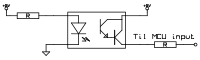
\includegraphics{./img/fotogaffel-diagram}
  \caption{Fotogafflens tilslutning til MCU}
  \label{fig:fotogaffel-diagram}
\end{figure}

Der ses på figuren~\vref{fig:fotogaffel-diagram} at vi har vores 5V
forsyning, hvor vi sætter en formodstand til lysdioden. Lysdioden vil
lyse hele tiden. Så afhængig af om man fører en fane ind eller ej, vil
vi få et logisk høj eller lav signal vi kan tolke vores MCU.

Man kunne evt. også bare tilslutte lysdioden til et output på MCU'en,
for at kunne tænde sensoren, når vi har brug for det i stedet for den
er tændt hele tinden. Men det spiller ikke megen rolle, da vi har har
en fast strømforsyning til plotteren.

\begin{figure}[htbp]
  \centering
  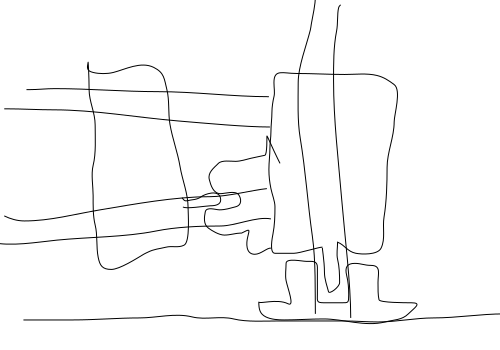
\includegraphics[width=7cm]{./img/fotogafel-skitse}
  \caption{Placering af fotogafler skitseret, set oppe fra i
    et hjørne af plotteren}
  \label{fig:fotogaffel-skitse}
\end{figure}

\section{SD-kort adapter}
Som følge af at vi har bestemt i vores kravspecifikation, at vi skal
kunne lægge data på et SD-kort, og få poltteren til at tegne det vi
har bestemt i dataene, så skal vi selvfølgelig også have lavet en
SD-kort adapter.

Ved at kigge på litteratur \cite{web:captain-mmc} og
\cite{web:sd-pinout}, har vi konstrueret en SD-kort adapter, som vi kan bruge
til vores ATmega128 print.

\begin{figure}[htbp]
  \centering
  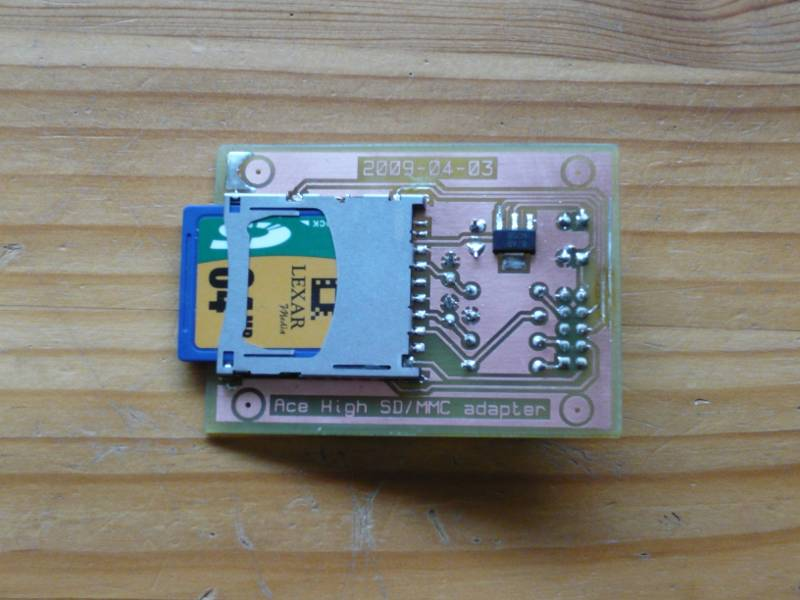
\includegraphics[width=7cm]{./img/sd-adapter}
  \caption{Den endelige SD-kort læser}
  \label{fig:sd-adapter}
\end{figure}

Der er ikke så meget, at sige om SD-kort adapterens kredsløb, da det
blot er forbindelser til kommunikation med vores
MCU. Kredsløbsdiagrammet kan ses i bilag~\vref{ch:b-sd}.

Den består af en SD-kort sokkel, hvor vi har taget højde for
forbindelserne mellem SD-kortet og MCU'en, jævnfør argumenterne fra
designafsnittet~\vref{sc:sda}.

Vi har en 3,3V spændingsregulator, og tre spændingsdelere der er
tilsluttet signalerne \textit{fra} vores MCU. Da SD-kortet som nævnt
ikke kan holde til de 5V vores MCU opperer ved.

\section{Tegnehoved}
Tegnehovedet har den fuktion, at den skal kunne løfte og sænke
pennen. Detter gør vi ved, at aktivere og deaktivere en
elektromagnet. Konstruktionen er beskrevet under
mekanikafsnitet~\vref{sc:i-tegnehovedet}.

Elektromagneten trækker meget strøm direkte forbundet (omkring 2A ved
20V). Vi har derfor valgt, at sætte en effektmodstand i serie med, for
at begrænse strømmen. Det er modstanden \texttt{R4} afbilledet i
figur~\vref{fig:tegnehoved-diagram}, på $47\Omega$. Valget på
$47\Omega$ er valgt vha. test. Vi har set hvilke effektmodstande vi
havde til rådighed, og så vurderet at den valgte var
passende. Selvfølgelig ved at tjekke om magneten er stræk nok.

\begin{figure}[htbp]
  \centering
  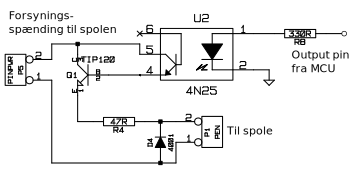
\includegraphics[width=11cm]{./img/tegnehoved-diagram}
  \caption{Styring til tegnehovedet}
  \label{fig:tegnehoved-diagram}
\end{figure}

Vi aktiverer vores sænker ved at sende et logisk høj signal til vores
tegnehoved afbryder. Den virker ved, at vi med et høj signal fra vores
MCU slutter optokobleren, hvorved den aktiverer \texttt{Q1}. Den åbner
hermed for strømmen, således den kan løbe gennem spolen.

%%% Local Variables: 
%%% mode: latex
%%% TeX-master: "../master"
%%% End: 
